\documentclass[ a4paper , 12pt ]{scrartcl}%%{article}

%% \usepackage[latin1]{inputenc}	%% schlecht für Umlaute
\usepackage[utf8]{inputenc}		%% erweiterter Eingabezeichensatz, bessere unterstützung von Umlauten
\usepackage[T1]{fontenc}		%% erweiterter T1 Zeichenvorrat
% \usepackage[ngerman]{babel}		%% Deutsche Übersetzung, Trennregeln
\usepackage[ngerman,english]{babel} % Main language: English
\usepackage{fancyhdr}			%% für Pagestyle fancyhdr mit eigenen Kopf und Fusszeilen
\usepackage{lmodern}			%% weiterenwicklung von Computer Modern
%\usepackage{a4wide}			%% nutzt das papier etwas besser
\usepackage{geometry}			%% etwas exaktere angaben der Seitenränder

\usepackage{amsmath}			%% Grundlegende Mathematikfunktionen
\usepackage{amssymb}			%%
\usepackage{amstext}			%% Text innerhalb von Gleichungen
\usepackage{amsfonts}			%%
\usepackage{mathrsfs}			%%
\usepackage{units}

\geometry{a4paper,left=25mm,right=25mm, top=25mm, bottom=25mm} 

\usepackage{pdfpages}

\usepackage{graphicx}			%%
\graphicspath{}				%%
\DeclareGraphicsExtensions{.png }	%% Portable Network Graphic.pdf} %% Portable Document Format

% \author{}

%% Pagestyle mit eigenen Kopf und Fusszeilen
\pagestyle{fancy}
\fancyhf{}				%% leerräumen
%\fancyhead[L]{\includegraphics[height = 20pt]{logo.png}}
% \fancyhead[R]{MSE/HSR Seminar Deep Learning}
\renewcommand{\headrulewidth}{0.0pt}	%% obere Trennlinie
\fancyfoot[L]{MSE/HSR Seminar Deep Learning}
\fancyfoot[R]{15 June 2017}	
% \fancyfoot[C]{}		
\renewcommand{\footrulewidth}{0.4pt}	%% untere Trennlinie

\begin{document}
% Very short summary of the very good LSTM description on http://colah.github.io/posts/2015-08-Understanding-LSTMs/ by Jonas Schmid

\center{ \textbf{\Large LSTM - Long Short-Term Memory}} \newline 
% \section*{ \center{ \textbf{\Large LSTM - Long Short-Term Memory}}}

\begin{figure}[h!]
	\centering
	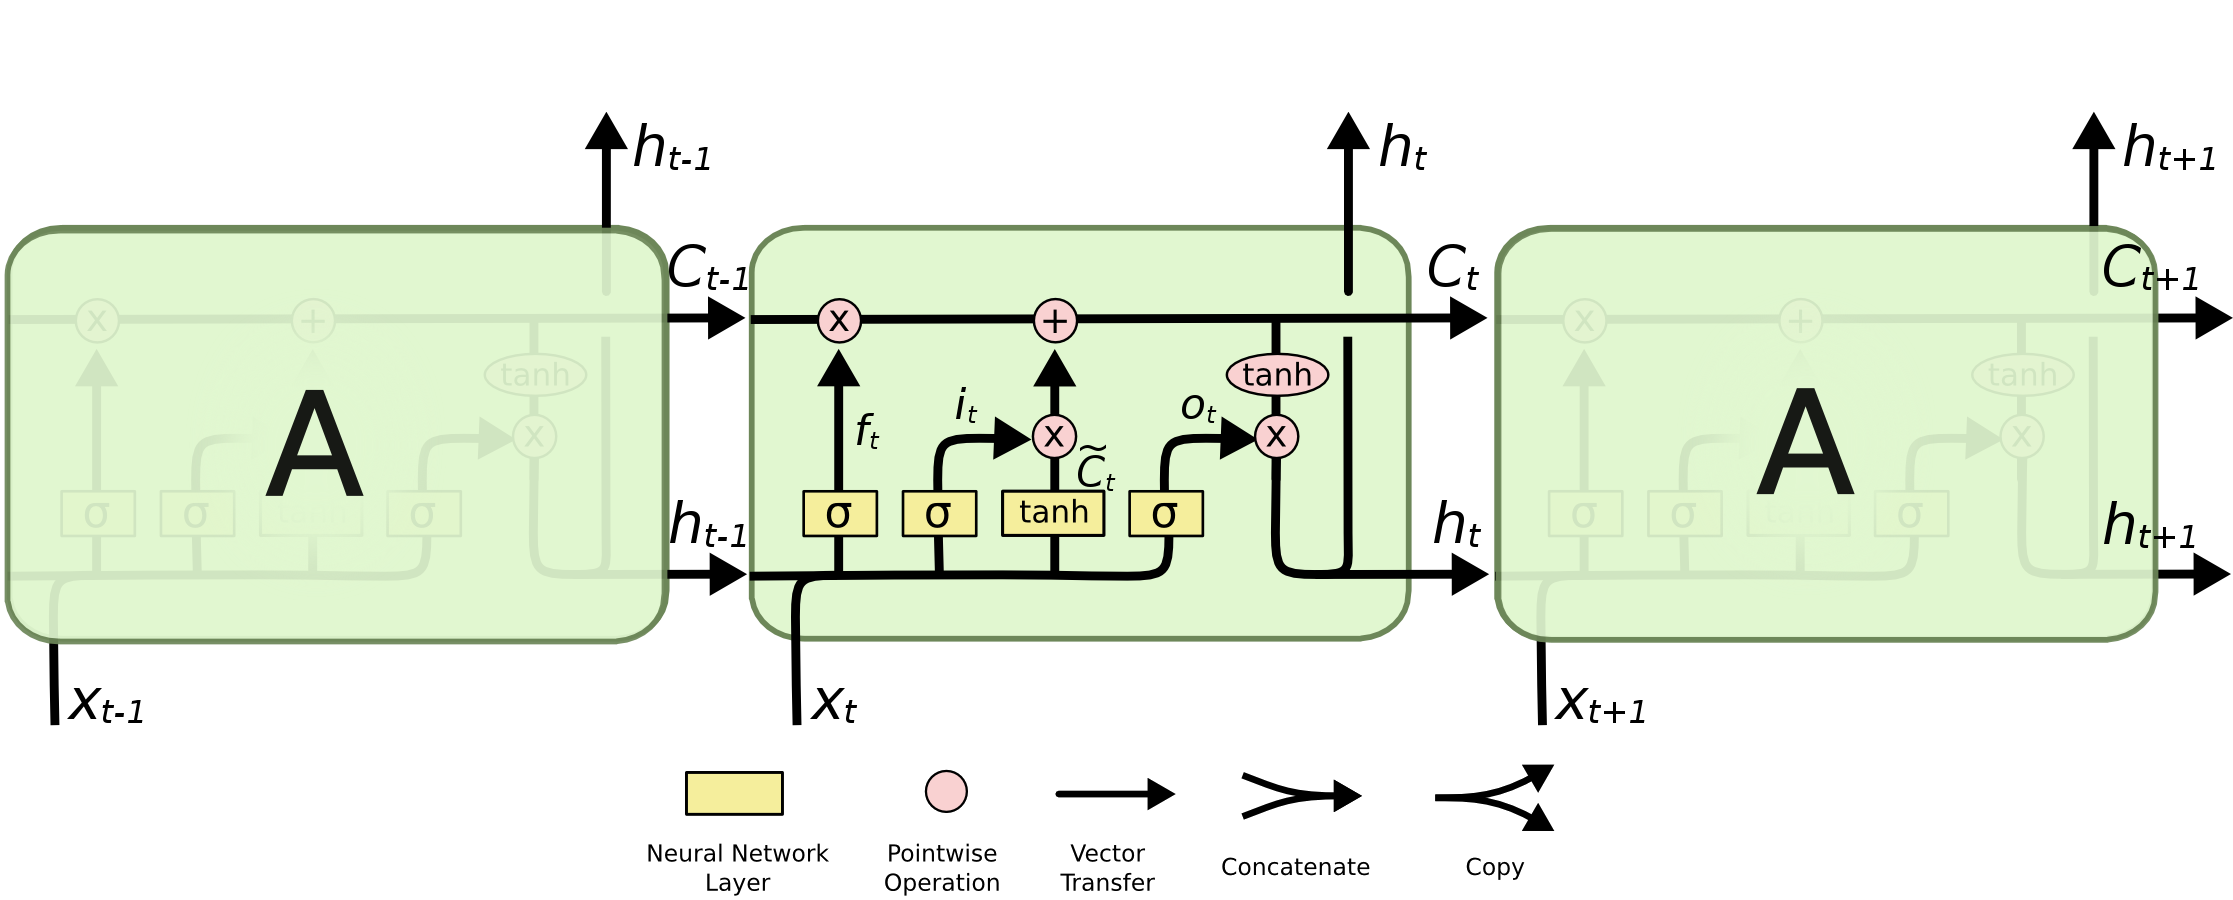
\includegraphics[scale=1.0, angle=0, clip ,trim= 200 0 200 40]{images/lstm_architecture_mod}
	\caption{Typical/Standard Long Short-Term Memory Cell Architecture (Source: http://colah.github.io/posts/2015-08-Understanding-LSTMs)}
	\label{fig:LSTMCell}
\end{figure}

\begin{itemize}
  \item[] $x_i$: Input data
  \item[] $C_i$: The cell state, this path through time is the key of LSTM architecture (Deep Learning Book: $s_i$). A kinde of a conveyor belt (Förderband).
  \item[] $h_i$: Hidden state similar to the standard RNN.
  \item[] $f_i$: Forget gate layer / path, rejects some information from the cell state.
  \item[] $i_i$/$\widetilde{C}_i$: What information of the input data will be stored in the cell state: Which information, a new candidate of information respectively (might inverted). Can be interpreted as a more complex and more powerfull input gate.
  \item[] $o_i$: Output gate, surpresses data from the cell state at the output (Deep Learning Book: $q_i$).
\end{itemize}

\begin{align}
f_t &= \sigma(W_f \cdot [h_{t-1},x_t] + b_f) \\
i_t &= \sigma(W_i \cdot [h_{t-1},x_t] + b_i) \\
\widetilde{C}_{t} &= tanh(W_C \cdot [h_{t-1},x_t] + b_C) \\
C_t &=  f_t \odot  C_{t-1} + i_t \odot \widetilde{C}_t \\
o_t &= \sigma(W_o \cdot [h_{t-1},x_t] + b_o) \\
h_t &= o_t \odot tanh(C_t)
\end{align}

\end{document}
